\documentclass{article}

% figures
\usepackage{graphicx}

% tables
\usepackage{booktabs}
\usepackage{pgfplotstable}
\usepackage{colortbl}
\usepackage{multirow}

% enumerations and bullets
\usepackage{paralist}

% references
\usepackage[numbers]{natbib}

% math
\usepackage{amssymb,amsmath,amsfonts}
\DeclareMathOperator*{\argmax}{argmax}

% algorithms
\usepackage[linesnumbered, ruled, vlined]{algorithm2e}
\SetAlFnt{\small}
\SetAlCapFnt{\small}
\SetAlCapNameFnt{\small}
\SetKwRepeat{Do}{do}{while}

% definitions and theorems
\usepackage{amsthm}
\theoremstyle{definition}
\newtheorem{definition}{Definition}
\usepackage{framed}

% listings
\usepackage{xcolor}
\usepackage{listings}
\definecolor{codegreen}{rgb}{0,0.6,0}
\definecolor{codegray}{rgb}{0.5,0.5,0.5}
\definecolor{codepurple}{rgb}{0.58,0,0.82}
\definecolor{backcolour}{rgb}{0.95,0.95,0.92}
\lstdefinestyle{mystyle}{
    backgroundcolor=\color{backcolour},   
    commentstyle=\color{codegreen},
    keywordstyle=\color{magenta},
    numberstyle=\tiny\color{codegray},
    stringstyle=\color{codepurple},
    basicstyle=\ttfamily\footnotesize,
    breakatwhitespace=false,         
    breaklines=true,                 
    captionpos=b,                    
    keepspaces=true,                 
    numbers=none,                    
%    numbersep=7pt,                  
%    numberstyle=\footnotesize,
    showspaces=false,                
    showstringspaces=false,
    showtabs=false,                  
    tabsize=2,
    frame=single,
    framesep=2pt,
    boxpos=c
}
\lstset{style=mystyle}

% color box
\usepackage{tcolorbox}

% etc
\usepackage[margin=3cm]{geometry}
\usepackage{setspace}

\setlength{\parindent}{0pt}  % no paragraph indentation (not recommended in general)
\setlength{\parskip}{6pt}    % space between paragraphs

% user commands for compiled annotations in PDF
\newcommand{\DS}[1]{{\color{red} [\textbf{DS}: #1]}}
\newcommand{\hl}[1]{\colorbox{green}{#1}}

\title{Latex Showcase (Evolving Document)}
\author{Donghwan Shin}
\date{\today}

\begin{document}

\maketitle

\section{Enumerations and Bullets}
Often we use enumerations and bullets in our papers. The following shows different ways to use them.

A basic style:
\begin{enumerate}
    \item First item
    \item Second item
    \item Third item
\end{enumerate}

This is a enumeration in a single line: 
\begin{inparaenum}[(1)]
    \item aaa,
    \item bbb, and
    \item ccc.
\end{inparaenum}

An enumeration with a custom label (especially useful in presenting research questions):
\begin{enumerate}[\bf RQ1]
    \item First RQ
    \item Second RQ
\end{enumerate}

A basic bullet listing:
\begin{itemize}
    \item First item
    \item Second item
\end{itemize}

A custom bullet listing:
\begin{itemize}[-]
    \item First item
    \item Second item
\end{itemize}


\section{Figures}

Figure~\ref{fig:parallel-boxplot} shows an example figure using centering.

\begin{figure}
	\centering
	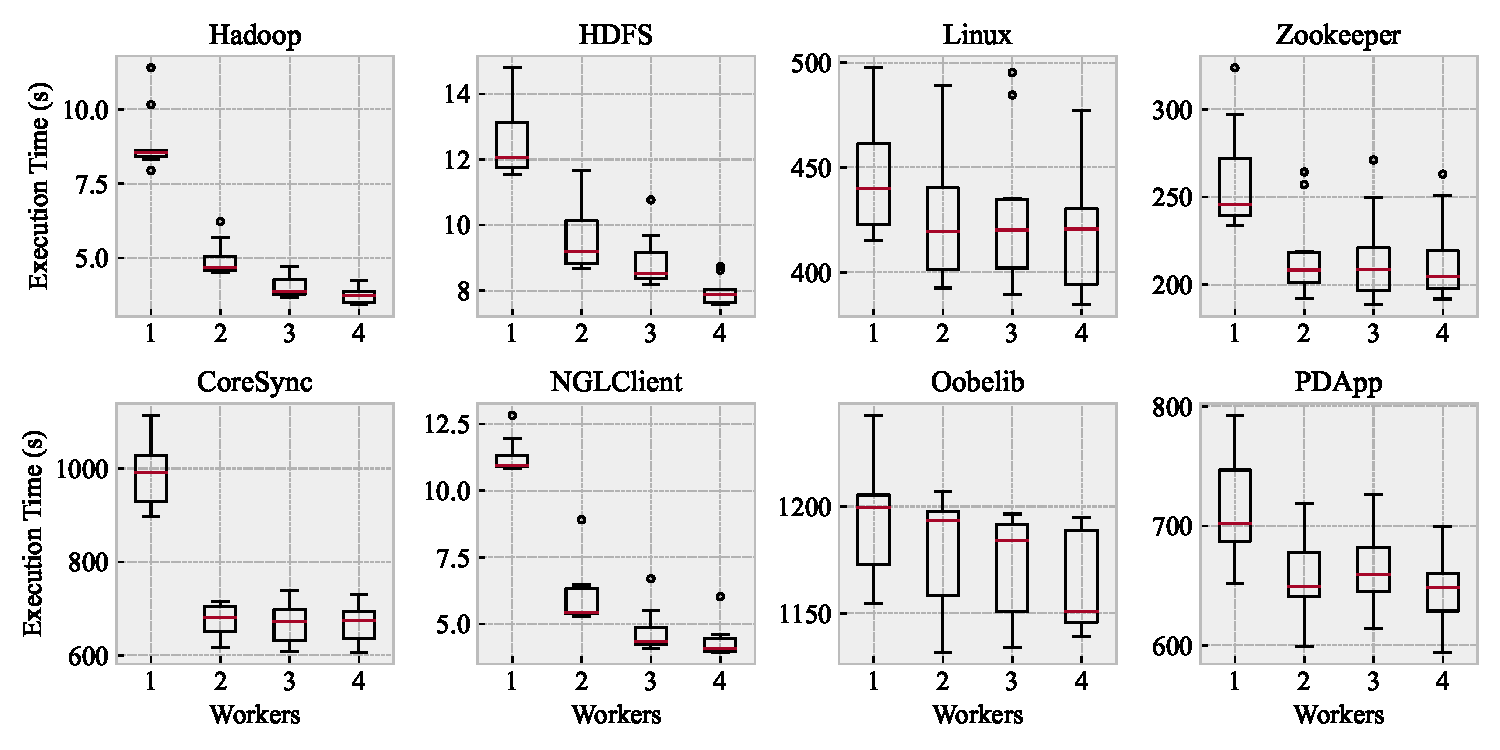
\includegraphics[width=\linewidth]{figures/rq1-boxplot.pdf}
	\caption{Relationship between the maximum number of parallel
          workers and the execution time of PRINS~\cite{shin2022prins}}
    \label{fig:parallel-boxplot}
\end{figure}


\section{Tables}

Table~\ref{table:subjects} is an example table using an external csv file and multirow.
Table~\ref{table:mint-prins-accr} is an example table using both an external data, multi-rows, coloured rows, and multi-columns. 

\begin{table}
\caption{Subject Systems and Logs~\cite{shin2022prins}}\label{table:subjects}
\centering
\pgfplotstabletypeset[
	col sep=comma,
	every head row/.style={before row=\toprule,after row=\midrule},
	every last row/.style={after row=\bottomrule},
	every row no 5/.style={before row=\midrule},
    columns/source/.style={
    		column type=l,
    		column name=Source,
    		string type,
	    assign cell content/.code={% use \multirow for type column:
			\ifnum\pgfplotstablerow=0
				\pgfkeyssetvalue{/pgfplots/table/@cell content}
					{\multirow{5}{*}{LogHub}}%
			\else
				\ifnum\pgfplotstablerow=5
					\pgfkeyssetvalue{/pgfplots/table/@cell content}
						{\multirow{4}{*}{PC}}%
				\else
					\pgfkeyssetvalue{/pgfplots/table/@cell content}{}%
				\fi
			\fi
		}
    },
    columns/system/.style={column type=l,column name=System,string type},
    columns/components/.style={column type=r,column name=\# Cmps},
    columns/logs/.style={column type=r,column name=\# Logs,1000 sep={\,},min exponent for 1000 sep=4},
    columns/templates/.style={column type=r,column name=\# Tpls},
    columns/entries/.style={column type=r,column name=\# Entries, 1000 sep={\,},min exponent for 1000 sep=4},
   	columns/confidence/.style={column type=r,column name=Conf,zerofill}
]{data/benchmark.csv}
\end{table}



\begin{table*}
\caption{Comparison between MINT (M) and PRINS (P) in terms of Accuracy. Differences between recall ($\Delta_R$), specificity ($\Delta_S$), and balanced accuracy ($\Delta_B$) values are expressed in percentage points (pp); $\mathcal{LDS}$ is the log-component diversity score~\cite{shin2022prins}.}\label{table:mint-prins-accr}
\centering
%\renewcommand{\arraystretch}{1.1}
\pgfplotstabletypeset[
	col sep=comma,
	%
	every head row/.style={before row={
		\toprule
		& \multicolumn{3}{c}{Recall} & \multicolumn{3}{c}{Specificity} & \multicolumn{3}{c}{Balanced Accuracy}\\
		\cmidrule(r){2-4} \cmidrule(r){5-7} \cmidrule(r){8-10}
	},after row=\midrule},
	every even row/.style={before row={\rowcolor{lightgray}}},
	every last row/.style={before row=\midrule, after row=\bottomrule},
	%
	fixed,fixed zerofill,precision=1,set thousands separator={},empty cells with={-},
	%
    columns/system/.style={column type=l,column name=System,string type},
    %
    columns/r_mint/.style={column type=r,column name=M,precision=2},
    columns/r_prins/.style={column type=r,column name=P,precision=2},
    columns/r_diff/.style={column type=r,column name=$\Delta_R$},
    %
    columns/s_mint/.style={column type=r,column name=M,precision=2},
    columns/s_prins/.style={column type=r,column name=P,precision=2},
    columns/s_diff/.style={column type=r,column name=$\Delta_S$},
    %
    columns/ba_mint/.style={column type=r,column name=M,precision=2},
    columns/ba_prins/.style={column type=r,column name=P,precision=2},
    columns/ba_diff/.style={column type=r,column name=$\Delta_B$},
    columns/lcdiv/.style={column type=r,column name=$\mathcal{LDS}$,precision=3,fixed}
]{data/rq5-table.csv}
\end{table*}


\section{Listings}

Figure~\ref{fig:example-program-slice} shows an example listing using the Python language semantic. 

\begin{figure}
\begin{lstlisting}[language=Python]
(2) db = DB.init(mode="default")
(4) item = getItem(db)
(6) if check(item) is "error":
(7)     logger.error("error in item: %s" % item)
\end{lstlisting}
\caption{Program slice $S_r$ of the program $P_\mathit{ex}$ when $s_7$ and its variable \texttt{item} are used as the slicing criterion~\cite{dawes2023towards}}
\label{fig:example-program-slice}
\end{figure}


\section{Algorithms}

\begin{algorithm}
\setstretch{1.35}
\SetKwInOut{Input}{Input}
\SetKwInOut{Output}{Output}

\Input{Input Domain $X$, \\
    Fitness Function $f: X \to Y$}
\Output{Best Solution $x_\mathit{best}\in X$ such that $x_\mathit{best} \approx \argmax_{x\in X}{f(x)}$}
    Best Solution $x_\mathit{best} \gets$ a candidate solution randomly sampled from $X$\\
     \While{$x_\mathit{best}$ is the ideal solution \textbf{or} we have run out of time}{
        Candidate Solution $x_c \gets$ a candidate solution randomly sampled from $X$\label{alg:sol}\\
        \If{$f(x_c) > f(x_\mathit{best})$}{
            $x_\mathit{best} \gets x_c$\\
        }
    }
    \textbf{return} $x_\mathit{best}$
\caption{Simple Random Search (for maximisation)}
\label{alg:mo}
\end{algorithm}

It is important to use the type information for each variable (e.g., ``Candidate Solution'' in front of $x_c$ in line~\ref{alg:sol}) since it significantly improves the readability of the algorithm. 


\section{Definitions and Theorems}

\begin{framed}
\begin{definition}[Log Parsing as an Abstraction Function]
Given a set of log messages $M$ and a generic set of parsing results $A$,
a log parsing approach can be represented as an abstraction function $\tau \colon M \to A$.
\end{definition}
\end{framed}

See \cite{rv2021} for more examples (and how to write a theoretical paper). 


\section{Coloured Box}

We often need to highlight some text in a coloured box, especially when we want to provide a compact summary of an evaluation result. The following shows how to do it.

\begin{tcolorbox}
    The answer to RQ1 is that ...
\end{tcolorbox}

\bibliographystyle{IEEEtranN} 
\bibliography{references} 

\end{document}
